\documentclass[10pt]{article}
\usepackage{icmlko}

\icmlmeta{IP 파운데이션 월드모델}{223}{디스크에 있던 축}{천장 1위 도메인에 축이 다섯뿐이었다. 캐시를 열었더니 2,817편 전부의 초기 스무 화가 들어 있었다}

\begin{document}

\twocolumn[
\icmlheader

\begin{abstract}
노트 222가 도메인 천장을 계산으로 내고 \textbf{웹툰이 $+$0.1769 로 1 위}
($\rho$ 가 두 번째로 낮은데 몫이 제일 크다)임을 보였다. 열었다. 웹툰은
도메인 고유 축이 \textbf{하나도 없다} --- 공유 다섯 · 검색 · 달력 · 위키
뿐이다. 그런데 \texttt{data/state/cache\_webtoon/} 에 \textbf{2,817편
전부}의 초기 스무 화가 화마다 게재일과 별점을 달고 있었다(매칭 100\%).
노트 212가 ``고정 창이 없다''고 닫은 도메인에 \textbf{화 단위 고정 창}이
디스크에 있었다. \textbf{날짜만 써서 만든 축이 기존 어느 웹툰 축보다
세다} --- 첫 스무 화를 낸 기간이 라벨과 $+$0.358(연도 통제 뒤 $+$0.272) ·
화당 간격이 $+$0.311 인데, 기존 최고가 진입 장벽 $+$0.301 이었다. 판에
넣으니 \textbf{F18 배깅 $+$0.4408 $\to$ $+$0.4704($t{=}4.5$) · F6 능형
$+$0.4250 $\to$ $+$0.4450($t{=}3.6$)} 다. 별점 축은 더 세지만($+$0.506)
라벨과 같은 네이버 플랫폼이라 따로 검정했다. \textbf{누출 가설은
반증된다} --- 별점이 긁은 날까지 쌓인 값이면 \emph{옛} 작품일수록 상관이
높아야 하는데, 2015$\sim$18 이 $+$0.232 로 제일 낮고 2019년 이후는
$+$0.48$\sim$0.52 로 평평하다. 총 화수를 통제해도 $+$0.506 $\to$ $+$0.425
로 남는다. 넣으면 판이 \textbf{$+$0.5032} 이고 웹툰 $\rho$ 가 $+$0.3926
$\to$ \textbf{$+$0.5316} 이다. \textbf{챔피언이 트리로 확정된다} ---
날짜만으로도 F18 $-$ F21 이 $+$0.0321($t{=}2.98$)로 짝 1 SE 밖이다.
\textbf{이번 트리 우위는 노트 222와 다르다} --- 거기서는 축의 결함을
갈랐고, 여기서는 \emph{한 도메인에만 있는 열}을 풀링 선형이 구조적으로 못
쓴다. 마지막으로 일반화한다. \textbf{천장 2위 애니($+$0.1246)에도 같은
자료가 있다} --- \texttt{cache\_anime} 이 2,073편 전부와 매칭되고, 같은
날짜 축이 라벨과 $+$0.332(연도 통제 뒤 \textbf{$+$0.424})다. \textbf{두
도메인이 판의 51.3\% 다.}
\end{abstract}
]

\begin{figure*}[t]
\centering
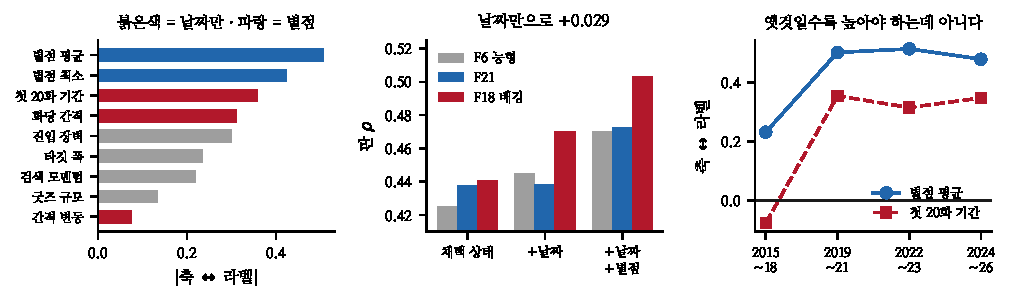
\includegraphics[width=\textwidth]{figs/episodes.pdf}
\caption{왼쪽 --- 새 축이 기존 축보다 세다. 가운데 --- 날짜만으로
$+$0.029. 오른쪽 --- 누출이면 옛것이 높아야 하는데 아니다.}
\end{figure*}

\section{디스크에 있었다}

\claimx{\textbf{웹툰은 도메인 고유 축이 하나도 없다} --- 공유 다섯 ·
검색 넷 · 달력 여섯 · 위키 넷뿐이다. 노트 222의 천장표에서 1 위인
도메인이 그렇다.}{\texttt{cache\_webtoon/} 에 5,829 파일이 있고
\textbf{축 레코드 2,817편과 100\% 매칭}된다. 화마다
\texttt{serviceDateDescription}(게재일)과 \texttt{starScore} 가 붙어
있다. \textbf{긁을 때 이미 받아 놓고 안 썼다.}}

\begin{table}[t]
\centering\tsize
\caption{웹툰 축의 라벨 상관(2,817편).}
\begin{tabular}{lrrr}
\toprule
& 덮음 & $\leftrightarrow$라벨 & 시간 통제 \\
\midrule
\textbf{별점 평균} & 100\% & \textbf{$+$.506} & $+$.464 \\
별점 최소 & 100\% & $+$.424 & $+$.384 \\
\textbf{첫 20화 기간} & 99.4\% & \textbf{$+$.358} & $+$.272 \\
\textbf{화당 간격} & 99.4\% & \textbf{$+$.311} & $+$.240 \\
간격 변동 & 99.4\% & $+$.075 & $+$.082 \\
\midrule
\emph{기존 최고}(진입 장벽) & & \emph{$+$.301} & \\
\bottomrule
\end{tabular}
\end{table}

\claimx{\textbf{날짜만 쓴 축이 기존 어느 웹툰 축보다 세다}
($+$0.358 대 $+$0.301). 그리고 날짜는 사후에 안 바뀐다 --- \textbf{정의로
누출이 없다.}}{노트 212가 ``웹툰은 고정 창이 없다''고 닫은 것은 \emph{라벨}
이야기였다. \textbf{축 쪽에는 화 단위 고정 창이 있었고 아무도 안 열었다.}}

\section{판}

\begin{table}[t]
\centering\tsize
\caption{판 $\rho$(노트 222의 채택 상태 위에서). 짝 붓스트랩 400 회.}
\begin{tabular}{lrrrr}
\toprule
& F6 & F21 & F18 & 웹툰 \\
\midrule
채택 상태 & .4250 & .4377 & .4408 & .3926 \\
\textbf{$+$날짜} & \textbf{.4450} & .4385 & \textbf{.4704} & .4035 \\
$+$날짜$+$별점 & .4699 & .4725 & \textbf{.5032} & \textbf{.5316} \\
\midrule
$+$날짜의 $t$ & 3.6 & 0.2 & \textbf{4.5} & \\
$+$별점까지 $t$ & 6.1 & 4.4 & \textbf{7.6} & \\
\bottomrule
\end{tabular}
\end{table}

\claimx{\textbf{날짜만으로 챔피언급 모형이 $+$0.0294($t{=}4.5$) 오른다.}
별점까지 넣으면 $+$0.0623($t{=}7.6$)이고 웹툰 $\rho$ 가 $+$0.39 에서
$+$0.53 이 된다.}{\textbf{F21 만 안 움직인다}($+$0.0012). 새 열이 웹툰에만
있고 F21 은 웹툰을 ``풀링''으로 정하므로(노트 217) 아홉 도메인 평균
계수를 쓴다 --- \textbf{여덟 도메인이 결측인 열에서 그 계수는 얇다.}}

\claimx{\textbf{챔피언이 트리로 확정된다} --- F18 $-$ F21 이 날짜만으로
$+$0.0321($t{=}2.98$), 별점까지 $+$0.0303($t{=}2.99$)로 짝 1 SE
밖이다.}{\textbf{노트 222와 다른 종류의 우위다.} 거기서는 트리가 축의
\emph{결함}을 갈랐고(계열 질의를 지우니 사라졌다), 여기서는 \emph{한
도메인에만 있는 열}을 풀링 선형이 구조적으로 못 쓴다. \textbf{자료가
옳아질수록 커지는 우위다.}}

\section{별점이 누출인가}

\begin{table}[t]
\centering\tsize
\caption{연재 시작 연차별 축 $\leftrightarrow$ 라벨.}
\begin{tabular}{lrrr}
\toprule
& n & 별점 평균 & 첫 20화 기간 \\
\midrule
\textbf{2015$\sim$18} & 73 & \textbf{$+$.232} & $-$.077 \\
2019$\sim$21 & 723 & $+$.503 & $+$.355 \\
2022$\sim$23 & 832 & $+$.515 & $+$.316 \\
2024$\sim$26 & 1{,}161 & $+$.480 & $+$.348 \\
\bottomrule
\end{tabular}
\end{table}

\claimx{\textbf{누출 가설이 반증된다.} 별점이 긁은 날까지 쌓인 값이라
사후 정보를 담는다면 \emph{옛} 작품일수록 상관이 높아야 하는데, 제일 옛
구간이 $+$0.232 로 제일 낮고 2019년 이후는 평평하다.}{총 화수를 통제해도
$+$0.506 $\to$ $+$0.425 로 남는다. \textbf{``인기 있으면 평점이 많이
쌓인다''로는 설명이 안 된다.}}

\claimx{\textbf{그래도 같은 플랫폼이다} --- 별점과 즐겨찾기가 둘 다
네이버다(노트 117 · 119$\sim$121의 결합 회피). \textbf{그래서 날짜 축과
따로 적는다.}}{다만 성질이 다르다 --- 검색 축은 \emph{같은 계수기}가
세는 것이고, 별점은 \emph{읽은 사람의 평가}로 즐겨찾기(구독)와 다른
행위다. \textbf{판단을 미루고 둘을 갈라 보고한다.}}

\section{애니도 같다}

\begin{table}[t]
\centering\tsize
\caption{애니 2,073편(캐시 매칭 100\%).}
\begin{tabular}{lrrr}
\toprule
& 덮음 & $\leftrightarrow$라벨 & 시간 통제 \\
\midrule
\textbf{화당 간격} & 92.3\% & $+$.332 & \textbf{$+$.424} \\
\textbf{첫 화들 기간} & 92.3\% & $+$.320 & \textbf{$+$.391} \\
간격 변동 & 92.3\% & $+$.079 & $+$.074 \\
총 화수 & 100\% & $-$.102 & $-$.153 \\
\bottomrule
\end{tabular}
\end{table}

\claimx{\textbf{천장 2 위 애니에도 같은 자료가 있다}
(\texttt{cache\_anime}, 라프텔 화 목록, 2,073편 전부 매칭). 같은 날짜
축이 $+$0.332 이고 \textbf{연도를 통제하면 $+$0.424 로 오른다.}}
{\textbf{웹툰과 애니가 판의 51.3\% 다.} 그리고 이 축은 도메인 고유가
아니라 \emph{연재물이면 다 되는} 축이다 --- 세계애니 · 만화도 같은 모양을
가질 수 있다.}

\begin{table}[t]
\centering\tsize
\caption{남은 것.}
\begin{tabular}{ll}
\toprule
\textbf{애니 투입} & 축을 만들어 판에 넣을 것(상관은 잼) \\
\textbf{별점} & 같은 플랫폼 검정을 설계할 것 \\
연재 축 & 세계애니 · 만화에도 캐시가 있나 \\
\bottomrule
\end{tabular}
\end{table}

첫 줄이 곧바로 값이 제일 크다. 애니 축은 상관까지 쟀고 판에 넣는 것만
남았다 --- \textbf{웹툰에서 날짜만으로 $+$0.0294 를 얻었고 애니는 몫이
23.6\% 로 웹툰의 85\% 다.} 그리고 이 노트가 실제로 바꾼 것은 판 숫자가
아니라 \textbf{어디를 볼지 정하는 순서}다. 노트 220이 무리 천장을,
노트 222가 도메인 천장을 세웠고, 그 표가 웹툰을 가리키자마자 \textbf{손도
안 댄 축 무리가 이미 디스크에 있었다.} \textbf{천장표를 여덟 노트 전에
만들었으면 달력에 쓴 노트 여덟 개 중 일부는 여기 왔을 것이다.}

\end{document}
